\documentclass{article}%
\usepackage[T1]{fontenc}%
\usepackage[utf8]{inputenc}%
\usepackage{lmodern}%
\usepackage{textcomp}%
\usepackage{lastpage}%
\usepackage[head=40pt,margin=0.5in,bottom=0.6in]{geometry}%
\usepackage{graphicx}%
%
\title{\textbf{“Chavismo originario” pide cambio de gobierno}}%
\author{Estefani Brito}%
\date{21/10/2018}%
%
\begin{document}%
\normalsize%
\maketitle%
\textbf{URL: }%
http://www.el{-}nacional.com/noticias/politica/chavismo{-}originario{-}pide{-}cambio{-}gobierno\_256579\newline%
%
\textbf{Periodico: }%
EN, %
ID: %
256579, %
Seccion: %
Política\newline%
%
\textbf{Palabras Claves: }%
NO\_TIENE\newline%
%
\textbf{Derecho: }%
18, %
Otros Derechos: %
CONTEXTO, %
Sub Derechos: %
\newline%
%
\textbf{EP: }%
NO\newline%
\newline%
%
\textbf{\textit{Wilmer Nolasco, Juan Barreto e Indira Urbaneja entregaron una carta en la OEA y su secretario general, Luis Almagro, aceptó reunirse con ellos para discutir la crisis}}%
\newline%
\newline%
%
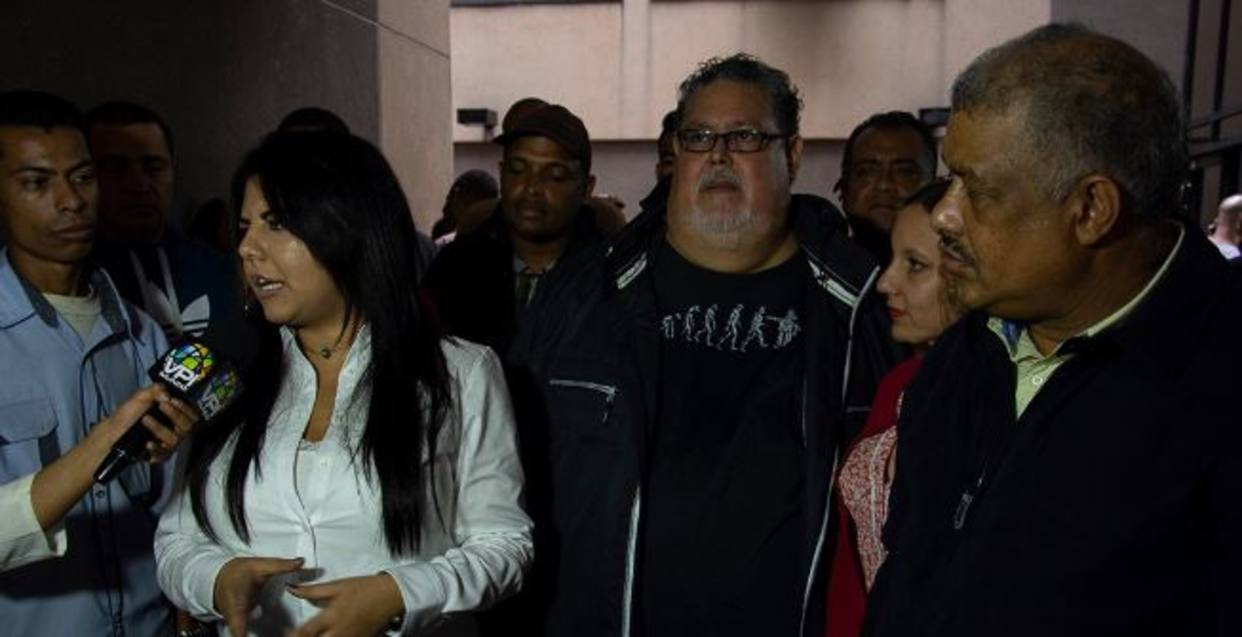
\includegraphics[width=300px]{141.jpg}%
\newline%
%
La Plataforma Alternativa Bolivariana y el Movimiento Chavismo Originario, representados por Wilmer Nolasco, Juan Barreto e Indira Urbaneja, rechazaron el “pastiche ideológico disfrazado de socialismo” que ostentan desde el poder quienes “intentan negar y minimizar una crisis que trastoca todos los ámbitos de la vida nacional”.%
\newline%
%
Pidieron que se dejara de colocar al “chavismo” en la misma categoría que al Ejecutivo, puesto que mezclan a “inocentes con corruptos, víctimas con victimarios y pueblo con cúpula”.%
\newline%
%
Esta plataforma se cataloga como oposición dentro del chavismo y en una carta consignada el viernes ante la sede de la Organización de Estados Americanos, en Caracas, denunció que el chavismo crítico –el que rechaza la ruptura del orden constitucional y el quebrantamiento de los derechos y libertades– es “perseguido, oprimido, chantajeado, amedrentado y calificado de traidor” por un gobierno que no admite crítica ni autocrítica.%
\newline%
%
El documento destaca que el grupo propone “un proceso de negociación, sincero, honesto y transparente que permita destrancar el juego político y asegurar una solución incluyente, pacífica y sostenible”.%
\newline%
%
Instaron al secretario general de la OEA, Luis Almagro, a que actúe como mediador y observador de un proceso de negociación amplio, con acompañamiento de organismos internacionales equilibrados e imparciales, en el que estén incorporados oposición, militares, el pueblo chavista y todos los sectores de la sociedad “que han sido invisibilizados”, con el fin de lograr un cambio pacífico y concertado de gobierno, e iniciar una transición que permita restaurar la Constitución, instituciones y poderes, y atender a los ciudadanos para alcanzar el equilibrio económico y social.%
\newline%
%
Además, de convocar a un proceso electoral con todas las garantías de ley que consideraron pero, no en estos momentos porque no es viable, dado que no existe una garantía de que los resultados serán aceptados.%
\newline%
%
En un tuit, Almagro respondió que reconoce al pueblo chavista “más allá de los horrores de la dictadura” y anunció que recibirá al “chavismo originario” en fecha acordada para discutir la crisis de Venezuela.%
\newline%
%
“Esta crisis no distingue colores partidistas, ni entre oposición y seguidores del gobierno; es de todos los venezolanos y eso incluye a los que venimos del chavismo, los que tenemos conciencia revolucionaria y democrática, que admitimos y asumimos con sentido crítico los errores y consecuencias de la desviación la Constitución de~1999”, sentenciaron.%
\newline%
%
\end{document}